% Metódy inžinierskej práce

\documentclass[10pt,twoside,slovak,a4paper]{article}

\usepackage[slovak]{babel}
%\usepackage[T1]{fontenc}
\usepackage[IL2]{fontenc} % lepšia sadzba písmena Ľ než v T1
\usepackage[utf8]{inputenc}
\usepackage{graphicx}
\usepackage{url} % príkaz \url na formátovanie URL
\usepackage{hyperref} % odkazy v texte budú aktívne (pri niektorých triedach dokumentov spôsobuje posun textu)

\usepackage{cite}
%\usepackage{times}

\pagestyle{headings}

\title{Porovnanie metód modelovania webových aplikácií\thanks{Semestrálny projekt v predmete Metódy inžinierskej práce, ak. rok 2021/22, vedenie: Vladimír Mlynarovič}} % meno a priezvisko vyučujúceho na cvičeniach

\author{Patrik Tomčo\\[2pt]
	{\small Slovenská technická univerzita v Bratislave}\\
	{\small Fakulta informatiky a informačných technológií}\\
	{\small \texttt{xtomco@stuba.sk}}
	}

\date{\small 16. októbra 2021} % upravte



\begin{document}

\maketitle

\begin{abstract}
%\ldots
Modely a modelovacie nástroje sú veľmi často používané softvérovými inžiniermi na vyjadrenie ich myšlienok počas vývoja softvéru. Tieto modely vedú k definícii modelovo-založeného vývojového procesu (MDD: Model-Driven Developement). Počas celej histórie softvérového inžinierstva boli pridávané nové využitia pre modely. Potenciálne benefity využívania modelov sú výrazne väčšie v softvérovej, ako v inej inžinierskej disciplíne.\cite{Selic:Pragmatics}. V MDE (Model-Driven Engineering) sú modely považované za hlavný vývojový artefakt na tvorbu softvéru. \cite{Gottardi:Metamodels}\\
Z toho môžme vyvodiť, že dôležitosť modelov v MDD je neodmysliteľná a je dôležité vedieť s nimi patrične narábať. 
Tento článok sa zaoberá popisom a porovnaním MDD metód, ktoré su esenciálne pre správne a dlhodobé fungovanie softvéru, ako aj pre jeho komplexnosť.
Taktiež analyzuje techniky navrhované na špecifikovanie funkčných, dátových a navigačných požiadaviek, ako aj poskytnutých mechanizmov na automatické preloženie týchto požiadaviek do koncepčných modelov. Hlavným cieľom tohto článku je preto pohľad a tieto metódy, využívaných vo vývoji webových aplikácií za účelom poukázania na ich silné a slabé stránky.\cite{Valderas:MDDE}\\
\\
Kľúčové slová: koncepčný model, modelmi riadený vývoj, metódy, webová aplikácia, modelmi riadené webové inžinierstvo, softvér
\\
\\ 
Čo pokladáte za významný problém v tejto oblasti a prečo (opora v literatúre)?\\

\end{abstract}


\section{Úvod}

Modelmi riadený vývoj (MDD: Model-Driven Developement) sa stáva stále viac a viac dôležitou a využívanou metódou vrámci softvérového inžinierstva. 
MDD tvrdí, že softvérové systémy musia byť vyvíjané pomocou modelov. MDD proces zvyčajne začína požiadavkovou fázou, v ktorej sa definujú požiadavkové modely, z ktorých následne vzikne jeden alebo viacero koncepčných modelov~\ref{KM}. Tie majú za úlohu popísať systém bez prihliadnutia na technologické aspekty softvéru a sú neskôr využité v analytickej fáze\cite{Valderas:MDDE}. Práve týmto modelom a metódam, v ktorých su obsiahnuté,  je venovaný tento článok. Presnejšie porovnaniu jednotlivých metód a koncepčných metód z nich pozostavujúcich. Tento článok sa zaoberá popísaním rôznych MDWE (Model-Driven Web Engineering) metód. Tieto metódy a koncepčné modely článok porovnáva z pohľadu MDD, ako aj z pohľdaju funkcionality a navigácie v rámci webových aplikácií a požiadaviek používateľa na spomenutých stránkach. V dnešnej dobe existuje enormné množstvo metód zaoberajúcich sa vývojom webových aplikácií. Preto by si popísanie všetkých metód dopodrobna vyžadovalo príliš veľké úsilie. Tento čánok sa preto venuje len redukovanje množine metód, aby bolo možné sa im viac dopodrobna venovať. Metódy, ktorým sa článok primárne venuje sú OOHDM(Obejct-Oriented Hypermedia Design Model), OOWS(Object Oriented Web Solutions) a WSDM(Web Site Design Method). Každá z týchto metód predstavuje koncepčné modely, ktoré nám umožnujú popísať webové aplikácie technologicky nezávislým spôsobom. "Tieto metódy boli úspešne aplikované vo vývoji viacerých webových aplikácií, čo je dôkazom toho, že implementácia konštruovania webových aplikácií pomocou koncepčných modelov a ich neskoršie prepísanie do kódu je možné".\cite{Valderas:MDDE}\\

Pre porozumenie tejto problematiky je veľmi dôležité vedieť, čo presne koncepčné modely predstavujú. Preto tento článok začne ich popisom. Ďalej bude pokračovať následovne. Sekcia 3 prezentuje prehľad popisovaných MDWE metód a ich bližší popis. Sekcia 4 sa venuje porovaniu týchto metód a koncepčným modelom z pohľadu MDD a funkcionality a navigácie v rámci  webových aplkácií. Sekcia 5 je venovaná metódam a modelom využivajúcim MDA (Model-Driven Architecture) prístup. Sekcia 6 slúži ako sumarizácia všetkého, čo sme zistili o danej problematike a sekcia 7 poskytuje prehľad bibliografie.\\
\\
Ešte spomenúť MDA prístup
\\
\section{Koncepčné modely} \label{KM}

Koncepčné modely webových aplikácií špecifikujú jej kompozíciu a navigáciu v nej\cite{Gkatouna:Patterns}. Kompozícia web stránky definuje, ktoré stránky tvoria hypertext a ich internú kompozíciu, ako aj možnosti používateľa na zaobchádzanie so systémom. Navigácia definuje rôzne spôsoby, ako môžu byť dané stránky navzájom prepojené linkami, ale aj zobrazenie postupnosti stránok, na základe používania zo strany používateľa, a obsahom vyobrazeným na stránke. Inými slovami, koncepčné modely webových aplikácií špecifikujú jej organizáciu jej front-end rozhrania v podobe stránok, dizajnových elexntov, ktoré sú prepojené linkami an uľahčenie navigácie na web stránke a manipulovania s ňou\cite{Gkatouna:Patterns}.

\section{Prehľad MDWE metód}

Následuje sekcia venujúca sa popísaniu troch vybraných MDWE (Model-Driven Web Development) metód. Tými sú, ako bolo spomenuté: OOHDM, OOWS , WSDM, Tieto metódy budú popísané chronologicky, podľa toho, v akom roku sa prvýkrát objavili v literatúre. Obrázok č.1 poukazuje na prehľad študovaných metód a chronologické usporiadnie podľa roku prvej publikácie. Tento článok sa venuje hlavne týmto metódam, pretože predstavujú techniky špeciálne vytvorené na špecifikovanie potrieb webových aplikácií.\cite{Valderas:MDDE}\\

\begin{figure*}[tbh]
\centering
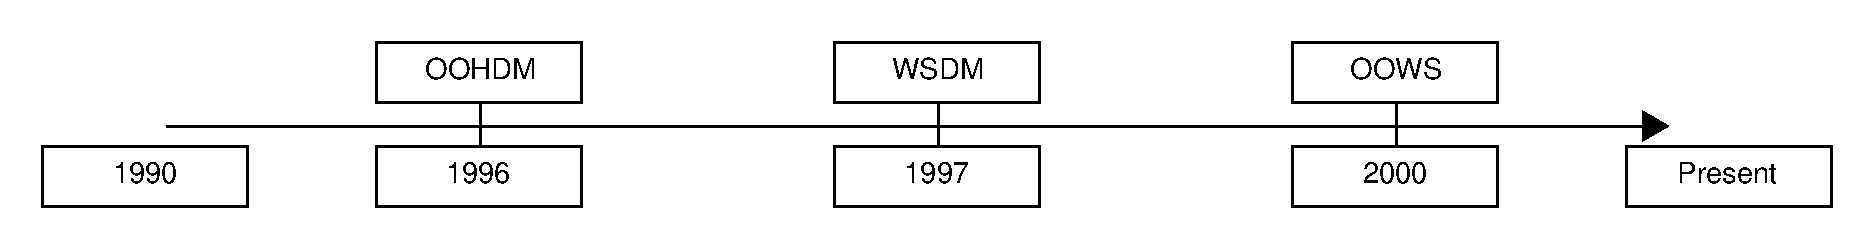
\includegraphics[scale=0.4]{Chronologický prehľad MDWE metód.pdf}.
\caption{Chronologický prehľad MDWE metód (upravený).}
\label{Prehľad}
\end{figure*}


\subsection{OOHDM: Object Oriented Hypermedia Design Model} \label{OOHDM}

OOHDM bolo vyvinuté pánmi Schwabe a Rossi v roku 1994. Bolo to jedno z prvých metodologických riešení pre vývoj webových aplikácií. OOHDM zdôrazňuje separáciu navigačných aspektov softvéru a od iných aspektov ako napríklad koncepčné aspekty a aspekty rozhrania. Ďalšie prístupy boli neskôr inšpirované touto myšlienkou separácií rôznych aspektov. "Nakoniec, je dôležité spomenúť, že OOHDM nie je uzatvorený prístup a je postupne rozširovaný a vylepšovaný."\cite{Valderas:MDDE}\\

Proces vývoja tohto prístupu je rozdelený do piatich hlavných fáz.

- Zhromažďovanie požiadaviek. V tejto fáze sú definovaný užívatelia, ktorý používajú webovú aplikáciu, ako aj uživateľské potreby, ktoré musí webová aplikácia podporovať.\\
- Koncepčný dizajn. Táto fáza pozostáva z koncepčnej schémy, v ktorej su popísané statické systémové aspekty.\\
- Navigačný dizajn. V tejto fáze musí byť definovaný diagram navigačných tried a diagram navigačnej štruktúry. Prvý reprezentuje statické možnostinavigačného systému. Druhý, na druhej strane, rozširuje prvý diagram vrátane prístupovej štruktúry a navigačného kontextu.\\
- Abstraktný dizajn rozhrania. Táto fáza definuje opis užívaťeľského rozhrania abstraktným spôsobom.\\
- Implementácia. V tejto fáze je webová aplikácia implementovaná. Táto implementácia je založená na predchádzajúcich modeloch.\\


\subsection{OOWS: Object Oriented Web Solutions} \label{OOWS}

Popísanie OOWS

\subsection{WSDM: Web Site Design Method} \label{WSDM}

Popísanie WSDM

\section{Porovnanie koncepčných modelov} \label{ina}

\section{Porovnanie koncepčných modelov vyžívajúcich MDA prístup}

\section{Zhrnutie}

\section{Bibliografia}


\section{Úvod1}

Toto je moj uvod\\
Prvy clanok\cite{Valderas:MDDE}. A druhy clanok\cite{Gkatouna:Patterns}.



Motivujte čitateľa a vysvetlite, o čom píšete. Úvod sa väčšinou nedelí na časti.

Uveďte explicitne štruktúru článku. Tu je nejaký príklad.
Základný problém, ktorý bol naznačený v úvode, je podrobnejšie vysvetlený v časti~\ref{nejaka}.
Dôležité súvislosti sú uvedené v častiach~\ref{dolezita} a~\ref{dolezitejsia}.
Záverečné poznámky prináša časť~\ref{zaver}.



Z obr.~\ref{f:rozhod} je všetko jasné. 

\begin{figure*}[tbh]
\centering
%\includegraphics[scale=1.0]{diagram.pdf}
Aj text môže byť prezentovaný ako obrázok. Stane sa z neho označný plávajúci objekt. Po vytvorení diagramu zrušte znak \texttt{\%} pred príkazom \verb|\includegraphics| označte tento riadok ako komentár (tiež pomocou znaku \texttt{\%}).
\caption{Rozhodujúci argument.}
\label{f:rozhod}
\end{figure*}






\section{Nejaka cast}
Základným problémom je teda\ldots{} Najprv sa pozrieme na nejaké vysvetlenie (časť~\ref{ina:nejake}), a potom na ešte nejaké (časť~\ref{ina:nejake}).\footnote{Niekedy môžete potrebovať aj poznámku pod čiarou.}

Môže sa zdať, že problém vlastne nejestvuje\cite{Coplien:MPD}, ale bolo dokázané, že to tak nie je~\cite{Czarnecki:Staged, Czarnecki:Progress}. Napriek tomu, aj dnes na webe narazíme na všelijaké pochybné názory\cite{PLP-Framework}. Dôležité veci možno \emph{zdôrazniť kurzívou}.



\subsection{Nejaké vysvetlenie} \label{ina:nejake}

Niekedy treba uviesť zoznam:

\begin{itemize}
\item jedna vec
\item druhá vec
	\begin{itemize}
	\item x
	\item y
	\end{itemize}
\end{itemize}

Ten istý zoznam, len číslovaný:

\begin{enumerate}
\item jedna vec
\item druhá vec
	\begin{enumerate}
	\item x
	\item y
	\end{enumerate}
\end{enumerate}


\subsection{Ešte nejaké vysvetlenie} \label{ina:este}

\paragraph{Veľmi dôležitá poznámka.}
Niekedy je potrebné nadpisom označiť odsek. Text pokračuje hneď za nadpisom.



\section{Dôležitá časť} \label{dolezita}




\section{Ešte dôležitejšia časť} \label{dolezitejsia}




\section{Záver} \label{zaver} % prípadne iný variant názvu



%\acknowledgement{Ak niekomu chcete poďakovať\ldots}


% týmto sa generuje zoznam literatúry z obsahu súboru literatura.bib podľa toho, na čo sa v článku odkazujete
\bibliography{literatura}
\bibliographystyle{plain} % prípadne alpha, abbrv alebo hociktorý iný
\end{document}
